\documentclass[nobib]{tufte-handout}
% \documentclass[fleqn,reqno,12pt]{article}

%========================================
% Packages
%========================================

\usepackage[nographicx, nohyperref, nosubcaption, nogb4e]{mfpackages}
\usepackage{mfenvironments}
\usepackage{mfcommands}
% for info boxes
\usepackage{newfloat, caption}
\DeclareCaptionType{InfoBox}


%========================================
% Bibliography
%========================================

\bibliography{references.bib}

%========================================
% General Layout Tweaks
%========================================

% \usepackage[margin=2cm]{geometry}

% Itemize
\renewcommand{\labelitemi}{\large{$\mathbf{\cdot}$}}    % itemize symbols
\renewcommand{\labelitemii}{\large{$\mathbf{\cdot}$}}
\renewcommand{\labelitemiii}{\large{$\mathbf{\cdot}$}}
\renewcommand{\labelitemiv}{\large{$\mathbf{\cdot}$}}
% Description
\renewcommand{\descriptionlabel}[1]{\hspace\labelsep\textsc{#1}}

% Figure Captions
\usepackage{caption} % use corresponding myfiguresize!
\setlength{\captionmargin}{20pt}
\renewcommand{\captionfont}{\small}
\setlength{\belowcaptionskip}{7pt} % standard is 0pt

%========================================
% Define colors and comment functions
%========================================

\usepackage{xcolor}
\definecolor{firebrick}{RGB}{178,34,34}
\definecolor{DarkGreen}{RGB}{34,178,34} 
\definecolor{DarkOrange}{RGB}{255,100,50}
\renewcommand{\mf}[1]{\textcolor{firebrick}{[mf: #1]}}  
\newcommand{\tr}[1]{\textcolor{DarkOrange}{[tr: #1]}}  
%========================================
% Configuring the R code presentation
%========================================

\usepackage{courier}
\usepackage{listings}
\usepackage{color}
% the following defines the layout for the R code
\lstset{ %
  language=R,                     % the language of the code
  basicstyle=\footnotesize\ttfamily, % size and type of the fonts that are used for the code
  numbers=left,                   % where to put the line-numbers
  numberstyle=\tiny\color{gray},  % the style that is used for the line-numbers
  stepnumber=0,                   % the step between two line-numbers. If it's 1, each line
                                  % will be numbered
  numbersep=5pt,                  % how far the line-numbers are from the code
  backgroundcolor=\color{white},  % choose the background color. You must add \usepackage{color}
  showspaces=false,               % show spaces adding particular underscores
  showstringspaces=false,         % underline spaces within strings
  showtabs=false,                 % show tabs within strings adding particular underscores
  frame=single,                   % adds a frame around the code
  rulecolor=\color{white},        % if not set, the frame-color may be changed on line-breaks within not-black text (e.g. commens (green here))
  tabsize=2,                      % sets default tabsize to 2 spaces
  captionpos=b,                   % sets the caption-position to bottom
  breaklines=true,                % sets automatic line breaking
  breakatwhitespace=false,        % sets if automatic breaks should only happen at whitespace
  title=\lstname,                 % show the filename of files included with \lstinputlisting;
                                  % also try caption instead of title
  keywordstyle=\color{black},      % keyword style
  alsoletter={_},                  % this treats _ as a letter
  commentstyle=\color{DarkGreen}, % comment style
  stringstyle=\color{DarkOrange}, % string literal style
  escapeinside={\%*}{*)},         % if you want to add a comment within your code
  morekeywords={*, ...},           % if you want to add more keywords to the set
  deletekeywords={_}         % remove keywords from list
}

% this is for showing the R output
\lstnewenvironment{rc}[1][]{\lstset{language=R, stepnumber=1}}{}

% this is for inline R code
\newcommand{\ri}[1]{\lstinline{#1}}  %% Short for 'R inline'


%========================================
% Article Header 
%========================================


\title{Bayesian regression modeling (for factorial designs): A tutorial}
\author{Michael Franke \& Timo Roettger}
\date{}

%========================================
% Article Body
%========================================

\begin{document}
\maketitle

\begin{abstract}
  \noindent Generalized linear mixed models are handy tools for statistical inference, and Bayesian approaches to applying these become increasingly popular. This tutorial provides an accessible, non-technical introduction to the use and feel of Bayesian mixed effects regression models. The focus is on data from a factorial-design experiment. \\
  
  \medskip
  
  \noindent \textbf{This tutorial should take you about 1.5 hours.}
\end{abstract} \marginnote{We would like to thank Oliver Bott, Joseph Cassilas, Artur Czeszumski, Fabian Dablander, Judith Degen, Elisa Kreiss, and Bodo Winter for their invaluable comments and suggestions on an earlier draft.}

\section{Motivation \& intended audience}

This tutorial provides a very basic introduction to Bayesian regression modeling using R \citep{Manual}. We wrote this tutorial with a particular reader in mind. If you have used R before and if you have a basic understanding of linear regression, and now you want to find out what a Bayesian approach has to offer, this tutorial is for you. In comparison to other introductions \citep[e.g.][]{SorensenHohensteinb2016:Bayesian-linear}, this tutorial remains very conceptual. We don’t want to ``sell Bayes'' to you, and we do not want to scare you away with mathematical details. We just want to give you an impression of how a Bayesian regression analysis looks and feels. The tutorial covers the essential concepts and explains how to run and interpret the output of a Bayesian regression analysis using the wonderful R package \texttt{brms} written by Paul \citet{buerkner2016brms}.


\marginnote{This tutorial contains gray text boxes which contain additional background information.
The information is sometimes a bit technical but never absolutely necessary for understanding the main ideas.
So feel free to read or skip any of the text boxes to suit your needs.}

If you don’t have any experience with regression modeling, you will probably still be able to follow, but you might also want to consider doing a crash course. To bring you up to speed, we recommend the excellent two-part tutorial by Bodo \citet{Winter2013:Linear-models-a} on mixed effects regression in a non-Bayesian ---a.k.a.~frequentist--- paradigm. In a sense, this tutorial could be considered part three of the series started by Winter. We will for example use the same data set.

To actively follow this tutorial, you should have R installed on your computer (\url{https://www.r-project.org}).
Unless you already have a favorite editor for tinkering with R scripts, we recommend to try out RStudio (\url{https://www.rstudio.com}).
You will also need some packages,
%\marginnote[-1cm]{Remember that you can install a package called \texttt{XYZ} %with the command \texttt{install.packages("XYZ")}.}
which you can import with the following code:
\marginnote[-1cm]{All code and data for this tutorial is also
  available for download here:
  \url{https://tinyurl.com/bmr-tutorial}}

\begin{minipage}[]{\textwidth}
\begin{lstlisting}[language=R]
# package for convenience functions (e.g. plotting)
library(tidyverse)

# package for Bayesian regression modeling
library(brms)

# option for Bayesian regression models: 
# use all available cores for parallel computing
options(mc.cores = parallel::detectCores())

# package for credible interval computation
library(HDInterval)

# set the random seed in order to make sure 
# you can reproduce the same results
set.seed(1702)
\end{lstlisting}
\end{minipage}

\vspace{-0.5cm}

\section{Data, research questions \& hypotheses}
\label{sec:data}

This tutorial looks at a data set relevant for investigating whether voice pitch differs across female and male speakers, and whether it differs across social contexts (say: informal and polite contexts).
To load the data into your R environment, run the following code:
%
\marginnote{The data is originally from research
presented by \citet{WinterGrawunder2012:The-Phonetic-Pr}. It is used in the tutorials by \citet{Winter2013:Linear-models-a} as well, but here we `massaged' the data a bit, i.e., we renamed variables and removed a line with missing data.}
%

\begin{minipage}[]{\textwidth}
\begin{lstlisting}[language=R]
# load the data into variable "politedata"
politedata = read_csv("https://tinyurl.com/polite-data")
\end{lstlisting}
\end{minipage}

\vspace*{-0.5cm}

\noindent Type \ri{head(politedata)} and you should see the first lines of the
data:

\begin{minipage}[]{\textwidth}
\begin{rc}
> head(politedata)
   subject gender sentence context pitch
   <chr>   <chr>  <chr>    <chr>   <dbl>
 1 F1      F      S1       pol      213.
 2 F1      F      S1       inf      204.
 3 F1      F      S2       pol      285.
 4 F1      F      S2       inf      260.
 5 F1      F      S3       pol      204.
 6 F1      F      S3       inf      287.
\end{rc}
\end{minipage}

\vspace{-0.5cm}


\noindent This data set contains information about different subjects, with an anonymous identifier stored in variable \texttt{subject}.
Because voice pitch is highly dependent on gender (i.e. there are anatomical differences between women and men that affect voice pitch), the variable \texttt{gender} stores whether a subject is F(emale) or M(ale).
Subjects produced different sentences (stored in the variable \texttt{sentence}), and the experiment manipulated whether the sentence was produced in a polite or an informal context, indicated by the variable \texttt{context}. Crucially, each row contains a measurement of pitch in Hz stored in the variable \texttt{pitch}.

Often, we are interested in an \textbf{outcome variable} (also called response or dependent variable, here \texttt{pitch}). We want to know how this outcome variable behaves
across different conditions or groups, which we call \textbf{predictors} (also called independent variable, here \texttt{gender} and \texttt{context}). Before our data collection,
we might have formulated concrete predictions about the relationship between the outcome and predictors. Let's assume previous research suggests that pitch is an indicator of politeness. Informal speech is accompanied by higher pitch in both men and women. Because the physiological difference between men and women is very large, we also predict that even in informal contexts, men still have lower pitch than women in polite contexts. We formulate the following hypotheses:
% \marginnote{Notice that our hypotheses are formulated explicitly as comparisons of
%   means / averages. The statistical model we will use indeed compares means, and this is common
%   practice, albeit a particular assumption worth highlighting. Commonly, this assumption is implicit: For example we could simply formulate H1 as something like
%   ``Female speakers' pitch is lower in polite than informal contexts.'' }

\begin{enumerate}[{H}1:]
\item Female speakers have a lower average pitch in polite than in informal contexts.
\item Male speakers have a lower average pitch in polite than in informal contexts.
\item Male speakers have a lower average pitch in informal than female speakers have in polite contexts.
\end{enumerate}

\section{Exploring the data visually}

Figure~\ref{fig:BasicPlotData_data} displays the mean pitch values for each
sentence (semi-transparent points) across gender and context.
%
\marginnote{Extensive plotting is always recommended to start data analysis. You need to
  know your data inside out. Pictures often reveal relationships much better than
  numbers can.}
%
The solid points indicate the average pitch values across all sentences and speakers.
Looking at the plot, we can see that pitch values from female speakers are generally higher
than those from male speakers (points in the left column are higher than in the right column).
We also see that pitch values in the informal context are slightly higher than those in the polite context (orange points are
slightly higher than purple points).
% \marginnote{The code needed to generated the picture in
%   Figure~\ref{fig:BasicPlotData_data} is not reproduced here, but included in the script in the
%   resources for this tutorial: \url{https://github.com/michael-franke/bayes_mixed_regression_tutorial}}

\begin{figure}[t]
  \centering
    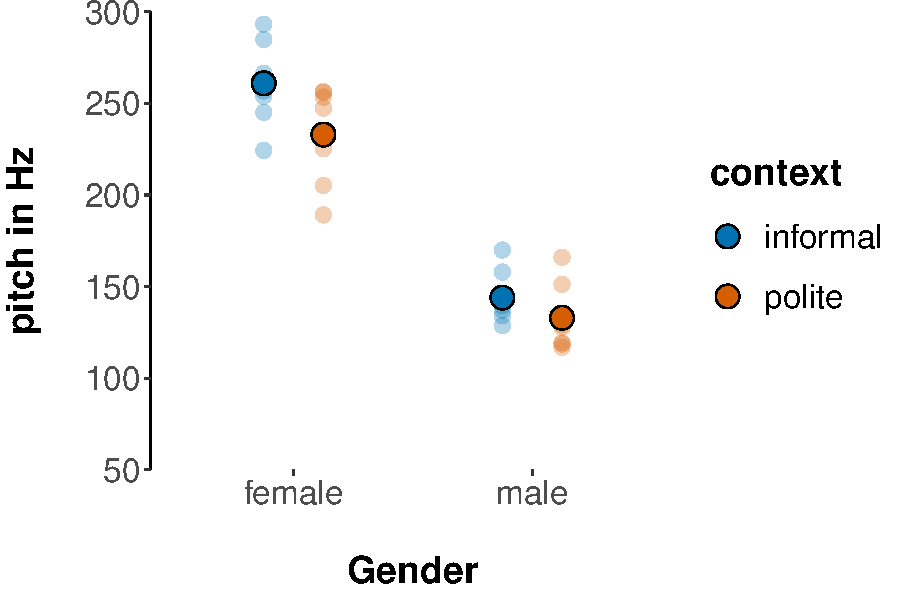
\includegraphics[width = \textwidth]{pics/basic_data_plot.pdf}
    \caption{Basic plot of the data displaying overall averages (thick points) and averages for individual sentences (smaller semitransparent points).}
     \label{fig:BasicPlotData_data}
\end{figure}


Looking at the plot, we might want to shout: ``The data confirm all of our hypotheses!'' But,
of course, we need to be more careful. As Bayesians, we would like to translate the data into
an expression of \textbf{evidence}: does the data provide evidence for our research hypotheses?
-- Also, notice that there is quite a lot of variability between different sentences (the
semi-transparent points in Figure 1). For example, some values from the informal condition for
female speakers (orange points in left column) are lower than their corresponding polite
counterparts. Similarly, there could be differences between individual speakers. What we want
are precise estimates of potential differences between conditions. We also want a measure of
how confident we can be in these estimates.

\begin{figure}[h]
  \centering
    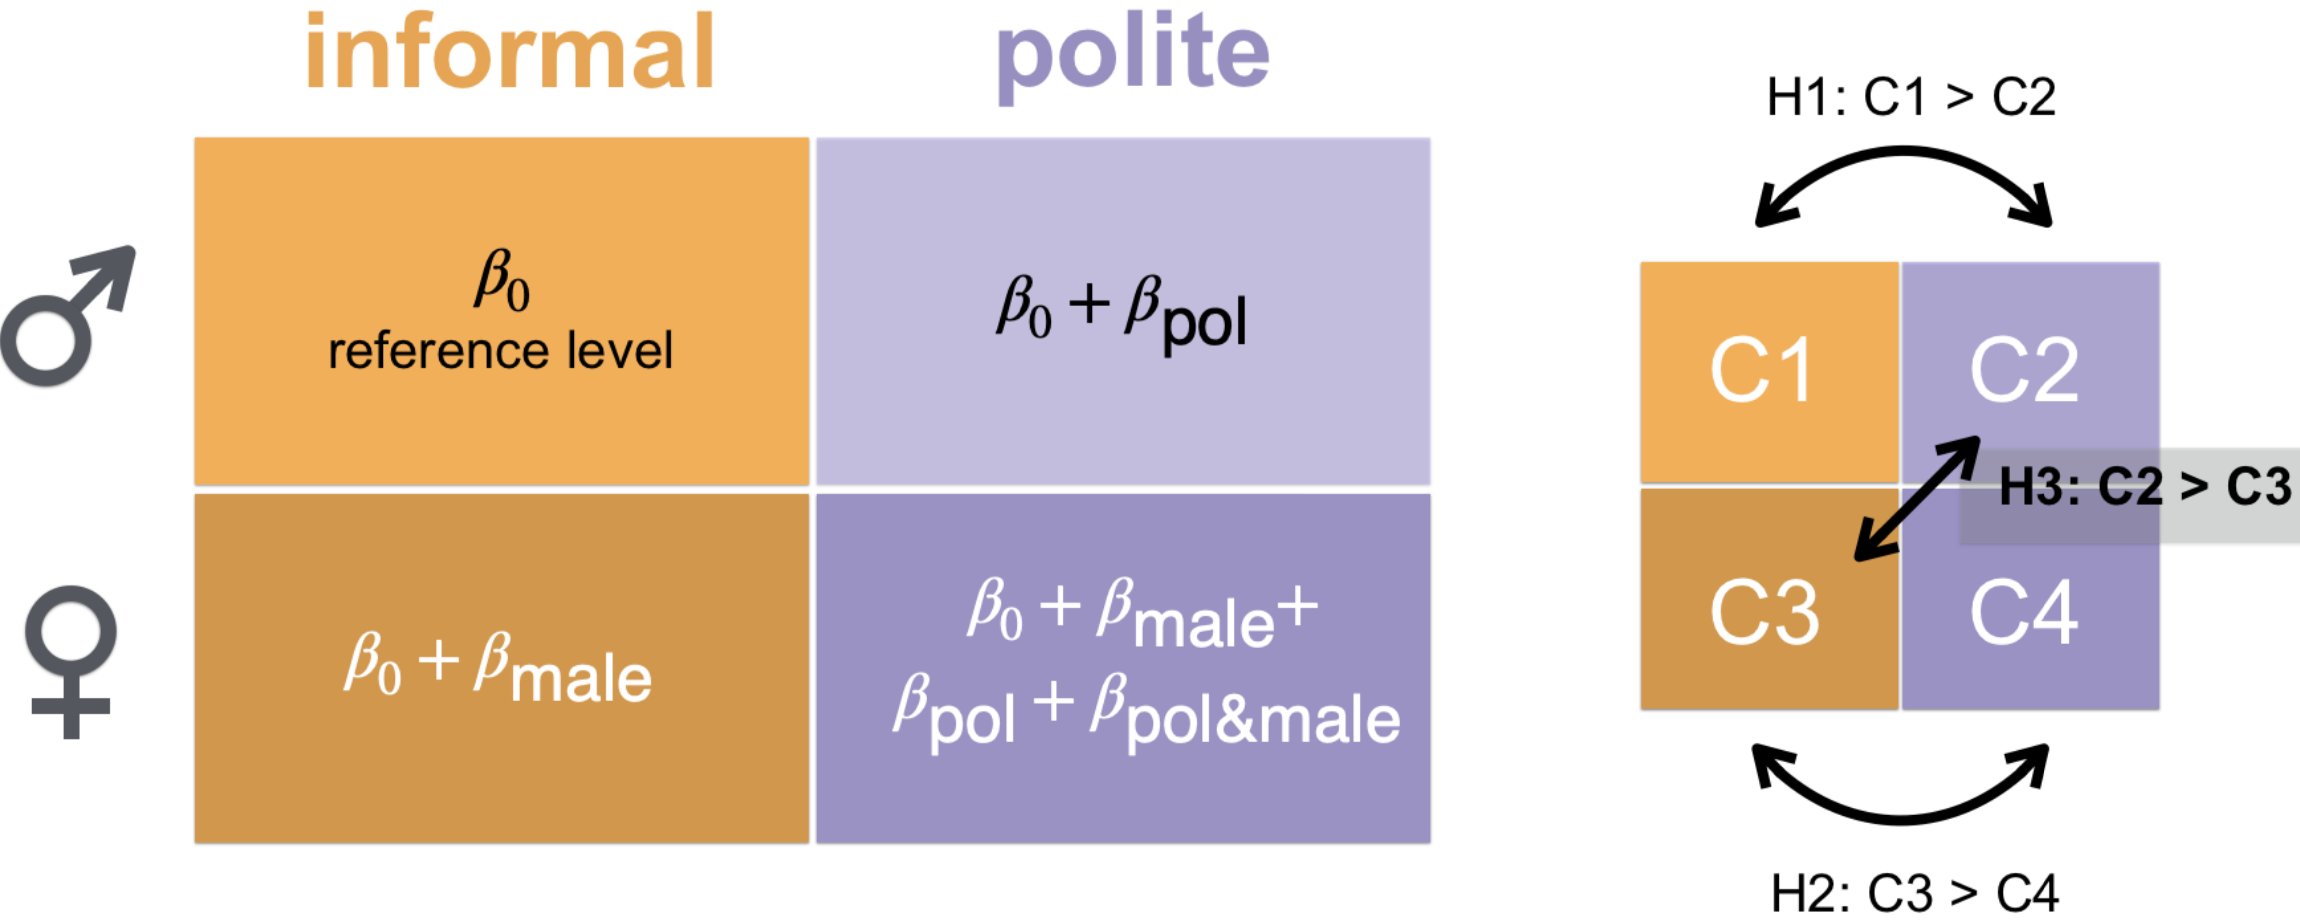
\includegraphics[width = \textwidth]{pics/table_mean_hypotheses_cropped.png}
    \caption{Coefficients of a dummy-coded regression model for the factorial $2 \times 2$ design, together with research hypotheses as statements about ordinal relations between cell means.}
    \label{fig:BasicPlotData_table}
\end{figure}

\section{A regression model for our data}

Another way of looking at the data in connection with our research hypotheses is displayed in
Figure~\ref{fig:BasicPlotData_table}. Each cell in this \textbf{design matrix} represents one
unique combination of the gender and the context factor.
%, and the table shows the mean of
%observed pitch values for each cell.
%
% \marginnote{In technical terms, this table is the \textbf{design matrix} of our experiment. We
%   have two factors of interest \texttt{context} and \texttt{gender}, each with two levels. The
%   table shows each combination of levels of all relevant factors. The cells in this table are
%   therefore also called \textbf{design cells} \tr{is this marginnote essential or can we maybe
%     get rid of it?}.}
%
Our hypotheses can be related to the comparison between the means of these cells.
H1 makes a statement about the comparison between C(ells) 1 and 2 (the context effect for female speakers); H2 makes a statement about C3 and C4 (the context effect for male speakers); and H3 makes a statement about C2 and C3 (the difference between informal male speakers and polite female speakers).

Before going into data analysis, let's look at the \textbf{regression model} we want to use.
%
\marginnote{The setup of this (non-hierarchical) regression model is not specific to a Bayesian approach. You would use the exact same for a frequentist analysis.}
%
Our regression model assumes that pitch values observed in each cell are
sampled from a population that is normally distributed around a mean, where each cell $c_i$ has its own mean $\mu_i$. We are interested in the probability of one cell mean being larger than another cell mean, i.e., the probability that $\mu_i > \mu_j$. Put differently, we are interested in the probability that the difference between $\mu_i$ and $\mu_j$ is larger than zero: $\mu_i - \mu_j > 0$.
%and since, let's say, it is easier to test whether a value is bigger than zero, we can encode the cell means like in Figure~\ref{fig:coefficients_table}. \tr{I cannot see this in the figure. The figure merely displays how we calculate the individual cell mean in a regression}
Figure~\ref{fig:BasicPlotData_table} illustrates the encoding scheme of our cell means in terms of a regression analysis. It assumes that
there is a \textbf{reference level} for each factor. Here it is the level \texttt{female} for
the factor \texttt{gender} and the level \texttt{informal} for the factor
\texttt{context}.\marginnote{This is so-called \textbf{dummy coding} (also referred to as \textbf{treatment coding}) of the regression
coefficients. Other coding schemes exist, but are not discussed here.} 
  
All cell means can then be expressed in terms of differences between the \textbf{intercept} aka our reference level
$\beta_0$, deviations from this reference level for each individual factor
($\beta_{\text{male}}$, and $\beta_{\text{pol}}$), and a so-called \textbf{interaction term}
$\beta_{\text{pol\&male}}$. In
other words, our regression estimates the mean of the reference level and estimates how much we
need to adjust this mean when we change either the context level (C2), the gender level (C3),
or both (C4). The $\beta$ terms are also called \textbf{coefficients}. They are \textbf{free parameters} of the model.

%\begin{figure}[]
%  \centering
%    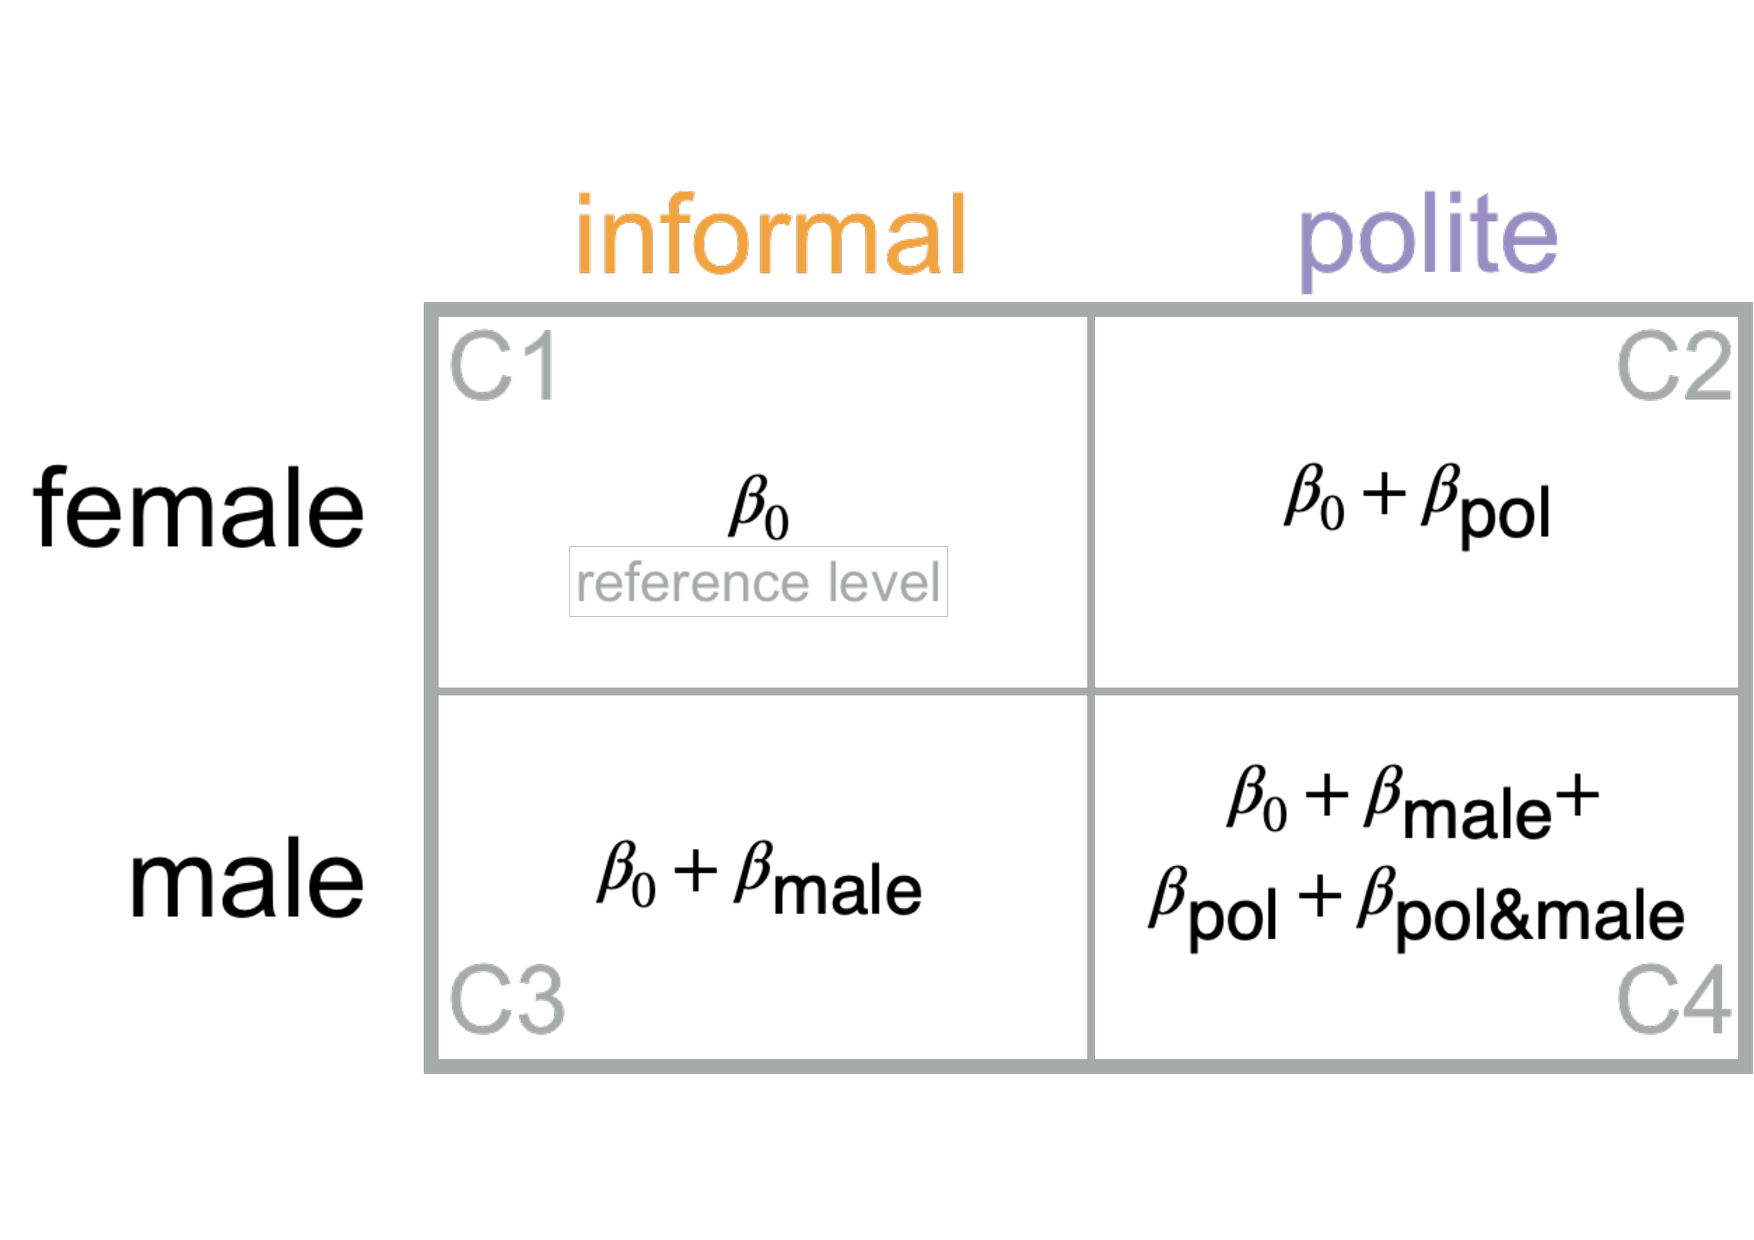
\includegraphics[width = 0.8\textwidth]{pics/table_coefficients.pdf}
%    \caption{Coefficients of a dummy-coded regression model for the factorial $2 \times 2$ design.}
%    \label{fig:coefficients_table}
%\end{figure}

%\begin{InfoBox}[]
%\centering
%\colorbox{mygray}{\centering
%  \begin{minipage}{1.0\textwidth}
%
%    \emph{Bayesian inference: priors, likelihoods and posteriors}
%    \medskip
%
%    Jones is a rational scientist and has recently become interested in speech patterns. She has read that women have higher pitch than men, but she is not quite convinced. She is determined to find out. How? Well, naturally, by rationally updating her
%    \emph{prior beliefs} about the pitch differences between men and women to obtain a new \emph{posterior belief} based on
%    empirical observation. Central to this updating is Jones'
%    \emph{likelihood function}, which encodes how likely any pitch difference may have generated the observed data.
%    
%    \paragraph{Prior beliefs.} Jones is a roll model scientist and starts from the prior assumption that there is no relationship between voice pitch and gender. She beliefs that men and women have the same voice pitch or in other words that the difference between male and female voice pitch is, on average at least, zero. Obviously she knows that nature is a messy beast, so she also departs from the assumption that this average difference varies a little bit on a case by case basis. She assumes that the average difference has a standard deviation of say 50.
%
%    \paragraph{Likelihood.} Let's assume that Jones takes a microphone and records five men and five women in front of her house. She measures their pitch values. Based on these data she can estimate the likelihood function (or simply likelihood). The likelihood is basically a function that maximizes the probability of getting an observed distribution.
%
%    \paragraph{Posterior beliefs.} Jones' measurements show a mean difference in pitch of 100 Hz and a standard deviation of 70 Hz. Her empirical observations suggest women have higher pitch values than men. Based on these observations, should she
%still believe that there is no difference between male and female pitch? By \emph{Bayes rule} her posterior beliefs are proportional to the product of her prior and the likelihood of her empirical observations.
%
%%\begin{figure}[]
%%  \centering
%%    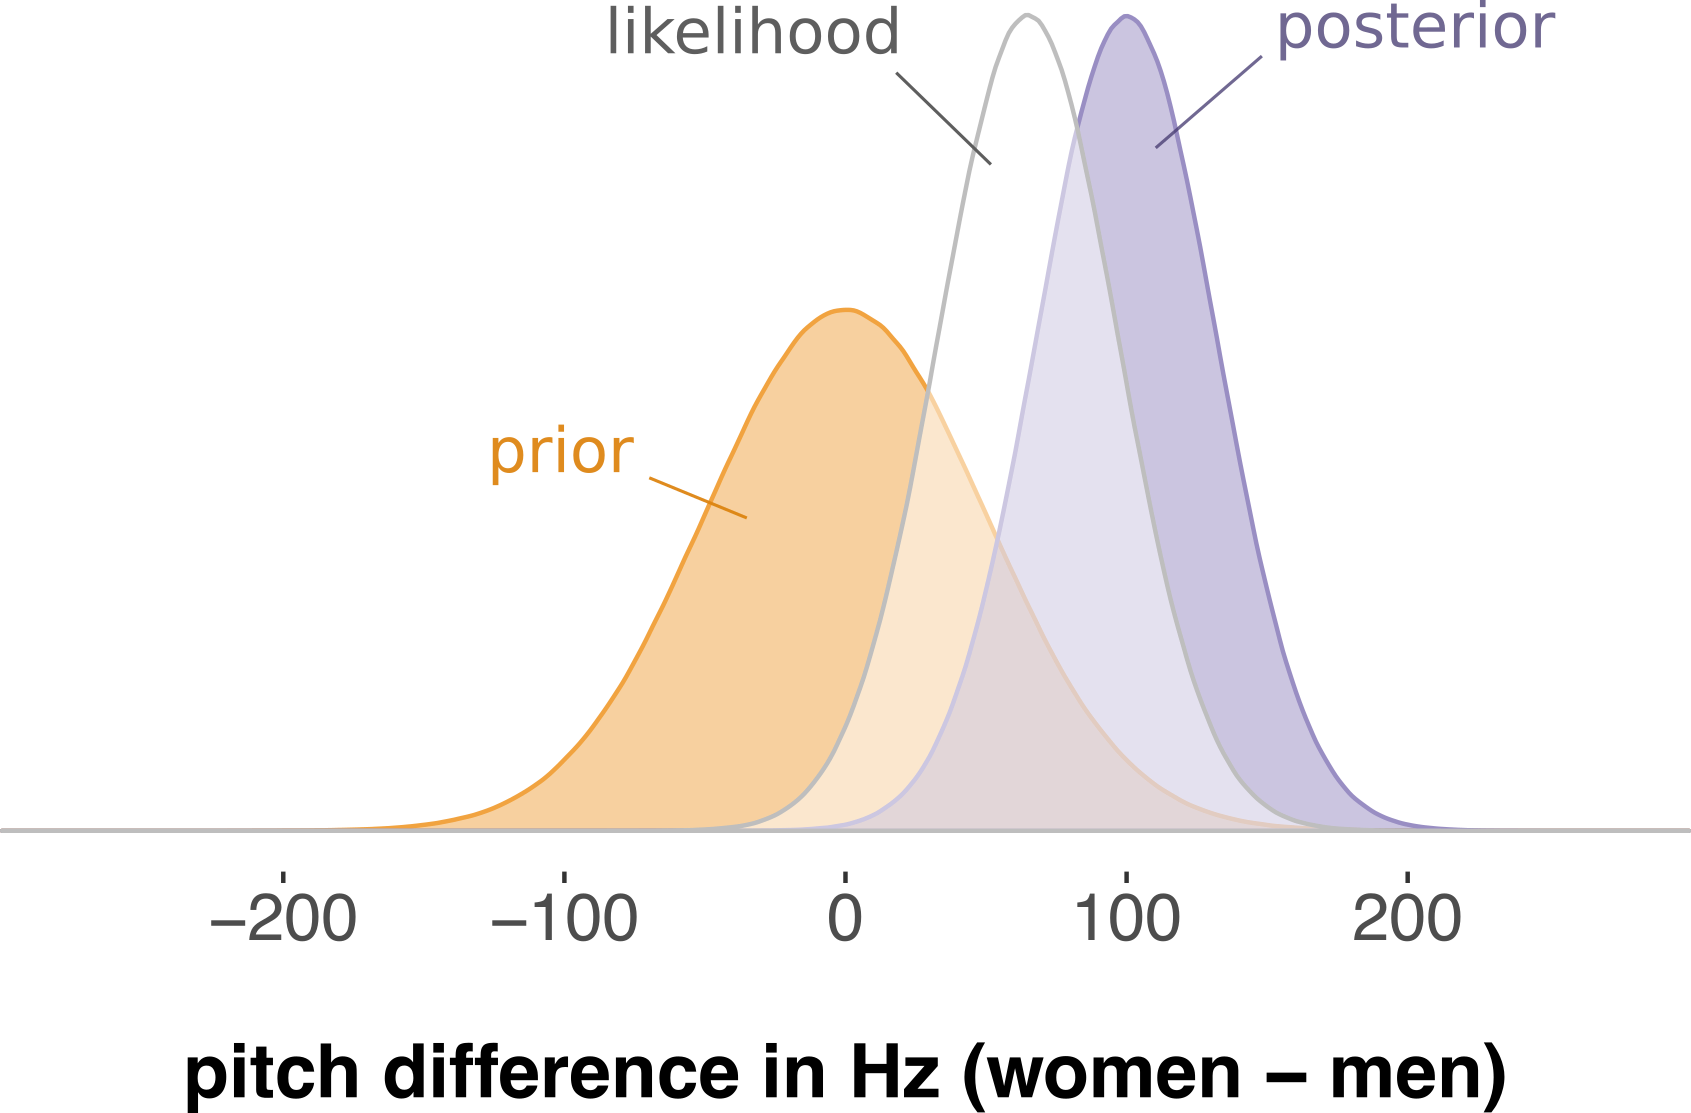
\includegraphics[width = 0.8\textwidth]{pics/prior_post.png}
%%    \caption{Possible relationship between prior, likelihood, and posterior. After observing the data, Jones  updates her prior and shifts her posterior beliefs towards the right.}
%%    \label{fig:prior_post}
%%\end{figure}
%
%\tr{possible to integrate the plot here? Well now that I look at it, this entire box might be redundant as you kinda talk about it in the next section. What do you think? Maybe cut?}
%    Jones' posterior belief in the voice pitch difference between men and women has shifted. After making her observation, rational Jones has updated her initial belief and is now more certain that there actually is a difference between men and women.
%    
%  \end{minipage} \par
%  } \par
%  \begin{center}
%    Info Box 1: Priors, likelihood and posteriors in Bayesian inference.
%  \end{center}
%  % \caption{\label{InfoBox:asymptotic_CIs} Here is my caption}  
%\end{InfoBox}


\section{A Bayesian analysis of a (fixed effects) regression model}

Having spelled out a model like the above, one way of testing our hypotheses in a Bayesian setting uses so-called \textbf{parameter inference}.
%
\marginnote[-2cm]{Another approach to testing hypotheses in a Bayesian setting is to use model comparison. This tutorial focuses on parameter estimation only for parallelism with the standard frequentist practice. We will briefly touch on model comparison at the end.}
%
Bayesian parameter inference asks: What should we believe about the values of the coefficients $\beta_0$, $\beta_{\text{pol}}$, $\beta_{\text{male}}$ and $\beta_{\text{pol\&male}}$ given the data, the model and whatever we believed before having seen the data? 
%Info Box~1 provides some background on Bayesian reasoning.


Formally, if $\theta$ is a vector of parameter values of the model, we are interested in the \textbf{posterior distribution} $P(\theta \mid D)$, which assigns a non-negative number to each tuple of parameters in proportion to how likely that tuple is.
From a Bayesian point of view, the model consists of a \textbf{likelihood function} $P(D \mid \theta)$, which specifies how likely an observation of data $D$ is for each value of parameters $\theta$, and a \textbf{prior distribution} $P(\theta)$, which specifies how likely we (the rational reasoner) believe each tuple of parameter values is in the first place.
%
\marginnote{Supplying a prior, really just \textit{any} prior, is important to get a
  Bayesian analysis off the ground; a circumstance which is discussed controversially. For many
  practical purposes, however, the precise choice of priors is not decisive and tools like the
  \texttt{brms} package (which we will use here) chooses generically reasonable default priors for the model (more on this below).}
%
With these ingredients, we can compute the posterior distribution by Bayes rule, as follows:
\begin{eqnarray*}
  P(\theta \mid D) = \frac{P(\theta) \ P(D \mid \theta)}{ \int P(\theta') \ P(D \mid
  \theta') \textrm{d}\theta'}
\end{eqnarray*}

%%%%%%%%%%%%%%%%%%%%%%%%%%%%%%%%%%%%%%%%%%%%%%%%%%%%%%%%%%%%%%%%%%%%%%%
%% Info Box 1
%%%%%%%%%%%%%%%%%%%%%%%%%%%%%%%%%%%%%%%%%%%%%%%%%%%%%%%%%%%%%%%%%%%%%%%

%\begin{InfoBox}[]
%\centering
%\colorbox{mygray}{\centering
%  \begin{minipage}{1.0\textwidth}
%
%    \emph{Bayesian inference: priors, likelihoods and posteriors}
%    \medskip
%
%    Smith claims that the mean pitch frequency of female Korean speakers is 130\,Hz. Miller claims that it is 160\,Hz. Jones is a rational scientist, and she wants to use data to inform her beliefs about whose theory is more likely correct. She does this by updating her prior beliefs via a likelihood function to obtain posterior beliefs.    
%   
%    \paragraph{Prior beliefs.} Jones' prior beliefs encode what she believes at the outset. She
%    considers two hypotheses, namely: H1, that the mean pitch of female Korean speakers is $\mu
%    = \mu_1 = 130$ and, H2, that it is $\mu = \mu_2 = 160$.  Jones initially believes that H1 is nine times more likely than H2 (for whatever reason), so that $P(\mu = \mu_1) = 0.9$ and, consequently, $P(\mu = \mu_2) = 0.1$.
%
%    \paragraph{Data.} Jones has recorded pitch frequencies of five speakers: \\ $D = \langle 140, 145, 150, 155, 160 \rangle$.
%    
%    \paragraph{Likelihood.} The likelihood function determines how likely any potential
%    observation is. It can depend on parameters, like the unknown $\mu$. In the case at hand,
%    let's assume that the data is generated by a normal distribution, with mean $\mu$ and a
%    fixed/known standard deviation $\sigma = 10$. The likelihood of the data is then $P(D \mid
%    \mu) = \prod_{i} \mathcal{N}(d_i, \mu, \sigma)$. This gives us $P(D \mid \mu_1) \approx
%    1.31e-12$ and $P(D \mid \mu_2) \approx 2.38-09$.
%
%     \paragraph{Posterior beliefs.} The data is more likely under the second hypothesis, but Jones initially considered the first more likely. Bayesian inference combines prior beliefs and likelihood. By \emph{Bayes rule} we compute the posterior probability of $\mu_1$ to be:
%     \begin{align*}
%       P(\mu_1 \mid D) = \frac{P(\mu_1) \ P(D \mid \mu_1)}{ \sum_{i =1}^2 P(\mu_i) \ P(D \mid \mu_i)} = \frac{0.9 \cdot 1.31e-12}{ 0.9 \cdot 1.31e-12 + 0.1 \cdot 2.38-09} \approx 0.005
%     \end{align*}
%     The data has very substantially changed Jones' beliefs: after rational belief update, she now considers H2 almost 200 times more likely than H1.
%     
%  \end{minipage} \par
%  } \par
%  \begin{center}
%    Info Box 1: Priors, likelihood and posteriors in Bayesian inference.
%  \end{center}
%  % \caption{\label{InfoBox:asymptotic_CIs} Here is my caption}  
%\end{InfoBox}

%%%%%%%%%%%%%%%%%%%%%%%%%%%%%%%%%%%%%%%%%%%%%%%%%%%%%%%%%%%%%%%%%%%%%%%

The R package \texttt{brms} \citep{buerkner2016brms} makes it easy to run Bayesian regression models. It uses a very similar formula syntax as related packages for regression analysis. In our case, we want to regress the dependent variable \texttt{pitch} against the independent variables \texttt{gender} and \texttt{context} and their two-way interaction. This model is expressed by the formula:

\begin{minipage}[]{\textwidth}
\begin{lstlisting}[language=R]
# formula for (fixed effects) regression model
formula_FE = pitch ~ gender * context
\end{lstlisting}
\end{minipage}

\vspace{-0.5cm}

The Bayesian model can then be fitted with the function \texttt{brm} from the \texttt{brms} package. We only need to specify the formula and supply the data. Here, we also set a seed to make sure we all produce exactly the same results.

\begin{minipage}[]{\textwidth}
\begin{lstlisting}[language=R]
# run regression model in brms
model_FE = brm(
  formula = formula_FE, 
  data = politedata, 
  seed = 1702 
)
\end{lstlisting}
\end{minipage}

\vspace{-0.5cm}

\noindent The \texttt{brms} package uses the probabilistic programming language \texttt{Stan}
in the background. \texttt{brms} basically translates our formula into Stan code that
implements a regression model and then executes it. The Stan code is then translated to C++
(hence the message about ``compiling C++'' when you run this code). Both the compilation in C++
and the sampling in Stan can sometimes take a while. It might also eat your battery in no time,
so always make sure your laptop is plugged in. Conceptually, Stan obtains samples from the
posterior distribution, based on an algorithm called \emph{Hamiltonian Monte Carlo}. This is an
instance of a more general class of algorithms, called \emph{Markov Chain Monte Carlo (MCMC)}
methods. The purpose of these methods is to return representative samples from the posterior
distribution. If you are interested in finding out more about this `sampling stuff', check out
Info Box~2.

\begin{InfoBox}[]
\centering
\colorbox{mygray}{\centering
  \begin{minipage}{1\textwidth}

    \emph{Markov Chain Monte Carlo (MCMC) sampling}
    \medskip
 
    Bayesian ideas are old, but they have recently seen a revival, mainly due to
    advances in computer science (notably: clever algorithms, not just faster computers). To
    understand this, consider Bayes rule for data analysis. We have a prior $P(\theta)$ over
    parameter $\theta$ and a likelihood function $P(D\mid\theta)$. We want to compute
    the posterior distribution:
    \begin{eqnarray*}
      P(\theta \mid D) = \frac{P(\theta) \ P(D \mid \theta)}{ \int P(\theta') \ P(D \mid
      \theta') \textrm{d}\theta'}
    \end{eqnarray*}
    If $\theta$ is a high-dimensional vector of parameters (e.g., in a hierarchical regression model), it
    might be quite impossible to compute the integral in the denominator. Fortunately, clever
    algorithms like MCMC allow us to draw \textbf{representative samples} from the
    posterior distribution without having to calculate the integral-of-doom.

    \medskip
    
    For common applications, it is not required to understand MCMC algorithms in full detail.
    It suffices to know that samples are collected by starting at (usually random) initial
    parameter values, and then ``jump around the parameter space'' in such a way that, if we
    were to jump infinitely often, we will have visited any particular tuple of parameter
    values with a relative frequency that corresponds exactly to its posterior probability. So
    these algorithms are guaranteed to give us representative samples, given unlimited time to
    jump around.

    \medskip
    
    To ensure the trustworthiness of a finite set of samples, we routinely run several
    \textbf{chains}, i.e., we start the ``jumping around'' procedure at different random
    initial starting points and check whether the different chains reached a similar outcome.
    We do this by plotting (so-called \emph{trace plots}) and the \textbf{$\hat{R}$-value}
    which is included in the \texttt{brm} model summary. An $\hat{R}$-statistic compares the
    variance of the samples within each chain to that from all samples across chains. If the
    $\hat{R}$-value is below 1.1, we commonly assume that the chains have converged
    sufficiently.

    \medskip
  
    In practice, the \texttt{brm} model summary and the messages during the fitting process will inform you about potential problems, and will normally offer good advice on how to solve the issue. 
   For example, sometimes the different chains do not converge on sufficiently similar results. 
    One quick and simple solution to these ``convergence issues'' is increasing the number of samples (specifying the option \texttt{iter} in the \texttt{brm} function call).
   
  \end{minipage} \par
  } \par
  \begin{center}
    Info Box 1: Background on sampling methods \& diagnostics.
  \end{center}
\end{InfoBox}


You can enter \texttt{model\_FE} in order to get a summary of the model fit. It should look like the following output.

\begin{minipage}[]{1.2\textwidth}
\begin{rc}
> model_FE
 Family: gaussian 
  Links: mu = identity; sigma = identity 
Formula: pitch ~ gender * context 
   Data: politedata (Number of observations: 83) 
Samples: 4 chains, each with iter = 2000; warmup = 1000; thin = 1;
         total post-warmup samples = 4000

Population-Level Effects: 
                   Estimate Est.Error l-95% CI u-95% CI Eff.Sample Rhat
Intercept            260.64      7.76   245.18   275.77       2148 1.00
genderM             -116.17     11.16  -137.71   -94.36       2115 1.00
contextpol           -27.43     11.11   -48.75    -6.36       1959 1.00
genderM:contextpol    15.83     15.87   -15.16    46.89       1975 1.00

Family Specific Parameters: 
      Estimate Est.Error l-95% CI u-95% CI Eff.Sample Rhat
sigma    36.14      2.81    31.09    42.08       4416 1.00

Samples were drawn using sampling(NUTS). For each parameter, Eff.Sample 
is a crude measure of effective sample size, and Rhat is the potential 
scale reduction factor on split chains (at convergence, Rhat = 1).
\end{rc}
\end{minipage}

\vspace{-0.5cm}

Lines 2--5 give us information about the model and the data used. Lines 6 and 7 tell us about
the sampling procedure (see Info Boxes~2 \& 3 for more information). Lines 9--14 contain information about our
parameters of interest. We will discuss them in detail below. Lines 16--18 contain information
that look similar to those in lines 9--14. This is the estimation of the standard deviation
\texttt{sigma}, describing the variance of the assumed normal distribution (which describe the
distribution of measures in each design cell). Finally, lines 20--22 contain general
information about the model fit and the information presented in this summary.
 \marginnote{If the model failed to converge or other problems occurred, you would see an informative message in the last part of this summary. See Info Box~2 for more on ``convergence''.}

Let us look at lines 9--14 in detail now. What these lines give us is a table with four rows, each of which corresponds to a parameter in the model, namely the coefficients shown in Figure~\ref{fig:BasicPlotData_table}. The variable \texttt{Intercept} refers to the coefficient $\beta_0$, which represents the mean of the reference level in cell 1 (female speakers in polite contexts). The variable \texttt{genderM} corresponds to the coefficient $\beta_{\text{male}}$, \texttt{contextpol} corresponds to the coefficient $\beta_{\text{pol}}$, and \texttt{genderM:contextpol} is the interaction coefficient $\beta_{\text{pol\&male}}$. For each of these parameters, the table contains very useful summary statistics based on the samples returned from the model fit.
%
\marginnote[-2.5cm]{Intuitively, the 95\% credible interval is the range of values that we can often practically consider credible enough to care about.}
%
More about the information given in the columns can be found in Info Box~3.

\begin{InfoBox}[t]
\centering
\colorbox{mygray}{\centering
  \begin{minipage}{1.0\textwidth}

    \emph{Information displayed in the summary of a \texttt{brm} model fit}
    \medskip

    Lines 6--7 of the summary of \texttt{model\_FE} tell us that we collected a total of 4000 samples from the posterior distribution. These came from four chains, each running for 2000 iterations, but discarding the first 1000 samples as \textbf{warm up}. We discard the first 100 samples because the initial starting point might be quite ``unrepresentative'' (see also Info Box~2).
    
    From the table in lines 9--14, the column \emph{Estimate} gives the mean of the obtained
    samples, thereby approximating the mean of the (marginal) posterior distribution for each
    parameter. For example, the parameter \texttt{Intercept} is estimated to have a mean of
    about $261$, which (here) coincides with the mean of the data points in cell 1, as shown in
    Figure~\ref{fig:BasicPlotData_table}. \emph{Est.Error} is the estimation error, an
    indication of the certainty we should have about the whole inference procedure. The columns
    \texttt{l-95\% CI} and \texttt{u-95\% CI} give the lower and upper bound of the 95\%
    credible interval for each parameter, as discussed in the main text. The column
    \texttt{Eff.Sample}, for efficient samples, gives us a rough measure of how many of all the
    samples we took (4000 in our case) are contributing non-redundant information to our
    estimation. The higher this number, the better. Finally, we get the \texttt{Rhat} column
    with the $\hat{R}$-values for each parameter (see Info Box~2).
    
  \end{minipage} \par
  } \par
  \begin{center}
    Info Box 2: Information in summaries of \texttt{brm} model fits.
  \end{center}
\end{InfoBox}


For our current purposes, the information in  columns \texttt{l-95\% CI} and \texttt{u-95\% CI} is most important.
These numbers give the lower and upper bounds of a \textbf{95\% credible interval}.
Take the parameter \texttt{contextpol}, corresponding to the coefficient $\beta_{\text{pol}}$.
This parameter corresponds to the estimated change of the mean of the reference level when we change the context level to polite.
The 95\% CI is roughly [-49;-6].
We could take values outside of this interval to be sufficiently unlikely to be ignorable for most purposes.
Consequently, this analysis suggests that zero is a very unlikely value for the coefficient
$\beta_{\text{pol}}$.
Given the data and the model, we should believe that $\beta_{\text{pol}}$ is most likely negative.
This directly addresses the first research hypothesis. Based on the regression model, the data suggests that H1 is likely true.

But how likely? How likely is it that $\beta_{\text{pol}}$ is smaller than zero? Instead of simply making a binary thumbs-up / thumbs-down decision, it would be even more elegant if we could put a number to it. As Bayesians we fortunately can. To see how this works, let us have a more intimate look at the samples that the \texttt{brm} function returns. We can access the samples of a model fitted with \texttt{brm} with the function \texttt{posterior\_samples}:

\begin{minipage}[]{\textwidth}
\begin{lstlisting}[language=R]
# extract posterior samples 
post_samples_FE = posterior_samples(model_FE)
head(post_samples_FE %>% round(1))
\end{lstlisting}
\end{minipage}

\vspace{-0.5cm}

The output of this could look like this:

\begin{minipage}[]{1.2\textwidth}
\begin{rc}
  b_Intercept b_genderM b_contextpol b_genderM:contextpol sigma   lp__
1       262.0    -117.6        -25.1                 13.5  38.8 -420.1
2       257.8    -118.9        -32.0                 12.6  37.6 -421.5
3       255.4    -114.4        -28.0                 11.4  37.2 -420.5
4       249.4    -101.1         -8.9                 -5.6  33.8 -421.0
5       283.4    -137.5        -46.1                 43.4  42.2 -425.4
6       284.8    -127.8        -45.8                 39.7  40.6 -427.6
\end{rc}
\end{minipage}

\vspace{-0.5cm}

What you see here is the top 6 rows of a data frame with columns for each parameter and 4000 rows, corresponding to each sample of that parameter (so the sampling method has generated 4000 values for each parameter, where each row is a sample from the posterior distribution $P(\theta \mid D)$).
%
\marginnote{The column \texttt{lp\_\_} contains the log-probability of the data for the parameterization in each row. This is useful for model comparison and model criticism but not important for our current adventures.}
%
We can use these samples to produce density plots reflecting our posterior distribution. The plot in Figure~\ref{fig:Posteriors_FE}
shows, for each of the four main model parameters, an estimate of the posterior density. Each
curve shows how much credence we should put on particular parameter values. For example, we see
that our beliefs concerning plausible values for the mean of cell 1 (female speakers in informal
contexts, the reference level) should hover around 260, roughly spreading from about 240 to 280.
We also see that all values that receive substantial probability density for \texttt{context:pol} (the coefficient $\beta_{\text{pol}}$) are negative (as captured in the 95\% CI discussed above). In other words,  the voice pitch of women in polite contexts is likely to be lower than in informal contexts. Zero is estimated to be a comparatively unlikely value for this parameter.

\begin{figure}
  \centering
  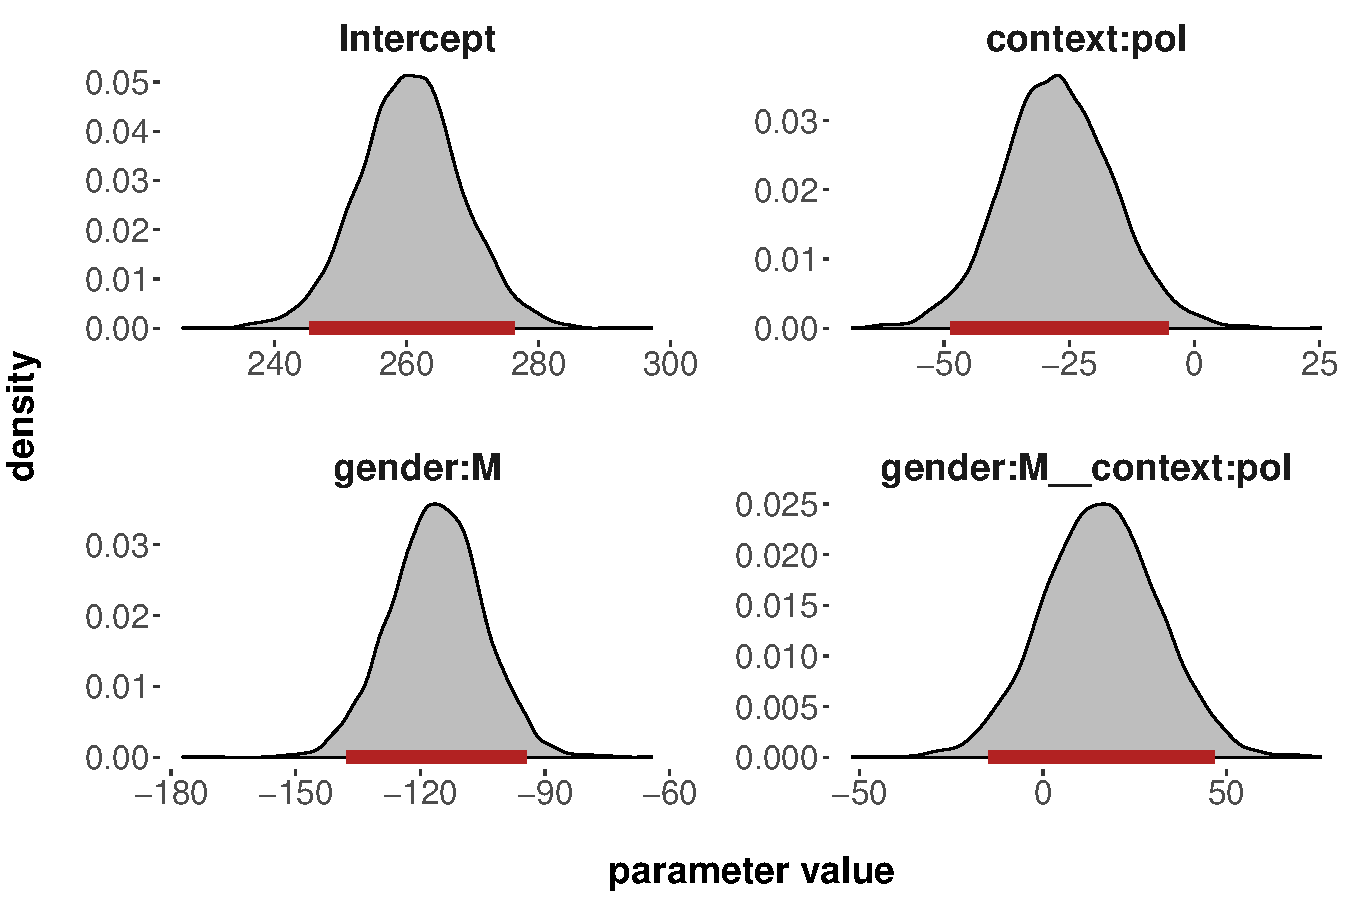
\includegraphics[width=\textwidth]{pics/posterior_density_FE.pdf}
  \caption[Posterior over coefficients in fixed-effects model]{Posterior density of parameter
    values in the fixed-effects regression model. The thick red lines indicate the 95\%
    credible intervals, i.e., the range of parameter values that it is reasonable to believe
    in.}
  \label{fig:Posteriors_FE}
\end{figure}

Now, here comes a nice gadget. Based on the samples obtained for \texttt{contextpol} ($\beta_{\text{pol}}$), it is very easy to estimate our belief that $\beta_{\text{pol}}$ is indeed negative. We simply have to calculate the proportion of samples that were negative. That's all. For instance, with the code below, which reveals that the posterior probability of the proposition that $\beta_{\text{pol}} < 0$ is about 0.99375. This is very close to 1!  

\begin{minipage}[]{\textwidth}
\begin{lstlisting}[language=R]
# proportion of negative samples for parameter b_contextpol
# this number approximates P(b_contextpol < 0 | model, data)
mean(post_samples_FE$b_contextpol < 0) 
>0.99375
\end{lstlisting}
\end{minipage}

\vspace{-0.5cm}

As an interim summary, we have seen how to run a Bayesian regression analysis with the
\texttt{brms} package and how to deal with its output. We have also seen that the output can be interpreted in very intuitive ways (e.g., ``The probability of H1, given our model, priors, and data, is more than .99'').

Unfortunately, what we have not seen yet is what the model and data say about hypotheses 2 or 3. This is because there is no single parameter in the (dummy-coded) regression model that corresponds to the differences between cells 3 and 4 (for hypothesis 2) and cells 2 and 3 (for hypothesis 3). Notice that this problem is not specific to Bayesian analyses, but inherent in the way the regression coefficients were set up.
%
\marginnote[-1cm]{A potential way of testing different hypotheses of the kind we have set out
  here, is to run different regression analyses, each with a different reference cell. This is
  a rather unhandy work flow. It wouldn't help with hypothesis 3 either, which compares the
  cell means in the design matrix ``diagonally'': there is no way of changing the reference level of either factor such that dummy coding gives us a single coefficient as the difference between cells 2 and 3.}
%
Fortunately, we can recover information about any derived measure from the obtained samples. Here's how:

Take hypothesis 3 which requires us to compare cells 2 and 3. The hypothesis states that
$\beta_0 + \beta_{\text{pol}} > \beta_0 + \beta_{\text{male}}$, which reduces to
$\beta_{\text{pol}} > \beta_{\text{male}}$. We can approximate the posterior probability that
this is true based on the samples that we obtained for the model in the same general way as
before, namely:

\begin{minipage}[]{1.1\textwidth}
\begin{lstlisting}[language=R]
# proportion of samples for which the mean of cell 2 was larger 
# than that of cell 3 
# this number approximates the quantity:
#    P(b_contextpol > b_genderM | model, data)
mean(post_samples_FE$b_contextpol > post_samples_FE$b_genderM)
>1
\end{lstlisting}
\end{minipage}

\vspace{-0.5cm}

Based on the posterior samples, the estimated probability is 1. That's a strong result. If the model was true, (given the data) our certainty that hypothesis 3 is true should be pretty much almost at ceiling.

To sum up, the Bayesian approach to regression modeling allows us to retrieve all direct comparisons between cells in a factorial design. It also allows us to retrieve quantitative information about our hypotheses in a way which is easy to communicate and understand. We can calculate the (estimated) posterior probability that a particular hypothesis holds. 

\section{The \texttt{faintr} package}

To make the comparison of pairs of cells even easier and applicable for even bigger factorial designs, this tutorial comes with a little R package, the \texttt{faintr} package.
%
% \marginnote[-1.5cm]{The name \texttt{faintr} is indicative of the possibility that the package might break down unexpectedly (we might consider renaming after more extensive testing), but also alludes to ``\emph{fa}ctorial design'' and ``\emph{int}erpretation'' somehow.}
%
You can install the package from GitHub with the \texttt{devtools} package, as follows:

\begin{minipage}[]{1.3\textwidth}
\begin{lstlisting}[language=R]
# load 'devtools' package to allow installation from GitHub
library(devtools)
# install 'faintr' package from GitHub
install_github(
  repo = "michael-franke/bayes_mixed_regression_tutorial", 
  subdir = "faintr")
# load the 'faintr' package
library(faintr)
\end{lstlisting}
\end{minipage}

\vspace{-0.5cm}

The \texttt{faintr} package provides two main helper functions.
%
\marginnote{More on the use of the \texttt{faintr} package can be found here: \url{https://tinyurl.com/faintr-vignette}.}
%
The function \texttt{post\_cells()}
takes as input the fitted regression model (technically: the \texttt{brmsfit} object returned
by function \texttt{brm}) and outputs samples for all design cell means, a comparison of all
design cells against each other, and a summary of each cell's inferred mean value.
For example, although the model fitted $\beta$-coefficients, we can reconstruct posterior estimates of each cell's means by typing:

\begin{minipage}[]{1.3\textwidth}
\begin{lstlisting}[language=R]
post_cells(model_FE)$predictor_values
\end{lstlisting}
\end{minipage}

\vspace*{-0.5cm}

\noindent Using these reconstructed samples, we can plot approximate posterior estimates for each cell, as in Figure~\ref{fig:Posteriors_cell_means}.

\begin{figure}
  \centering
  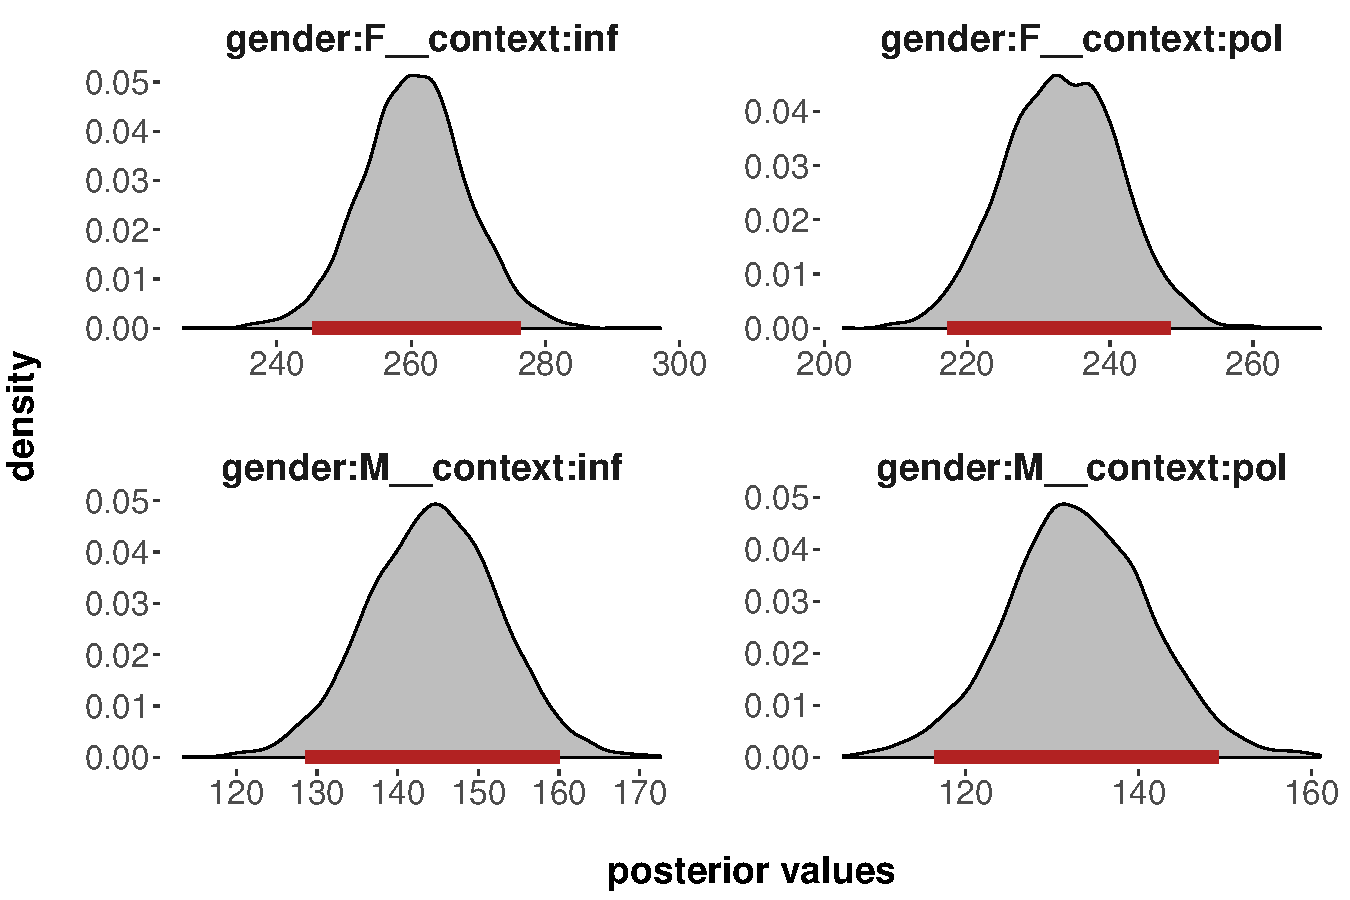
\includegraphics[width=\textwidth]{pics/posterior_density_cell_means.pdf}
  \caption[Posteriors over cell means in fixed-effects model]{Posterior density of cell means
    in the fixed-effects regression model. The thick red lines indicate the 95\% credible
    intervals, i.e., the range of parameter values that are reasonable to believe in (given the data and the model.}
  \label{fig:Posteriors_cell_means}
\end{figure}


Another helpful function is \texttt{compare\_groups()}, which takes the fitted regression model as input together with a specification of which two (subsets of) cells to compare
against each other. For example, we can compare (diagonally) the cells for female speakers in
polite contexts with male speakers in informal contexts with this call:

\begin{minipage}[]{1.3\textwidth}
\begin{lstlisting}[language=R]
compare_groups(
  model = model_FE, 
  lower = list(gender = "M", context = "inf"),
  higher = list(gender = "F", context = "pol")
)
\end{lstlisting}
\end{minipage}

\vspace{-0.5cm}

\noindent The output looks like this:

\begin{minipage}[]{\textwidth}
\begin{rc}
Outcome of comparing groups:
 * higher:  gender:F context:pol 
 * lower:   gender:M context:inf 
Mean 'higher - lower':  88.74 
95% CI: [ 68.09 ; 111 ]
P('higher - lower' > 0):  1 
\end{rc}
\end{minipage}

\vspace{-0.5cm}

For the purposes of this tutorial, we gather the output of the \texttt{compare\_groups()} for
all of the three hypotheses of current interest in a convenience function (which the interested
reader will find in the source code, but which is of no further theoretical interest here): 

\begin{minipage}[]{\textwidth}
\begin{rc}
> get_posterior_beliefs_about_hypotheses(model_FE)
# A tibble: 3 x 2
  hypothesis                      probability
  <chr>                                 <dbl>
1 Female-polite < Female-informal       0.994
2 Male-polite < Male-informal           0.849
3 Male-informal < Female-polite         1
\end{rc}
\end{minipage}

\vspace{-0.5cm}

Based on the currently assumed model and data, we would conclude that hypotheses 1 and 3 are very likely true, but we can also see that there is quite a bit of uncertainty associated with hypothesis 2. The probability of H2 (given the data and the model) is only 0.849. So we should be sufficiently suspicious about H2 until more evidence is available.

%
\marginnote{It is generically reasonable to consider posteriors above 0.95 or 0.975 as large enough to warrant speaking of ``evidence in favor of a hypothesis''.}

\section{Priors}

One important difference between frequentist and Bayesian inference are priors. Priors are pieces of information about our data that we assume before actually looking at them. Specifying priors has several advantages, both technical and conceptual. First, we can use \textbf{regularizing priors} to implement soft constraints on what counts as a plausible parameter setting for the model, thereby reducing the computational resources needed to estimate the model parameters.
%
\marginnote[-1.5cm]{Defining regularizing priors is essential for more complex models which have to estimate many parameters. Regularizing priors can help the model to converge more quickly.}
%
As a conceptual advantage, priors can also express relevant subjective prior beliefs about the situation or problem at hand. For example, pitch values (and many other things we measure in nature) cannot be smaller than zero. Human pitch values are also limited to a certain range defined by physiological and bio-mechanical constraints on our laryngeal system. In adults, values larger than, let's say, 1000 Hz are very unlikely. 
 
But wait a minute. Subjective beliefs? This is science. We are supposed to be objective, right?
We should have a heart of stone and be skeptical about possible relationships in the first
place. Practically, this means the following for us: We should not hesitate to make use of the
possibility to bring all the potentially relevant background knowledge to bear when analyzing
our data. The formalization of background knowledge should, of course, be made transparent and
be explicitly justified. So, any pieces of reasonably uncontroversial background knowledge
might well be included in the model. But, of course, when it comes to the specific hypotheses
we would like to test, we should \emph{not} engineer in the conclusions we would like to
eventually draw, no matter what our subjective beliefs (possibly inspired by hope) are! If our
research hypothesis is that female speakers lower their voices in polite contexts, we obviously
don't want to specify a prior that assumes the hypothesized relationship before having seen the
data. Instead, we can feed the model with a skeptical prior about the truth of our
research hypothesis. Since there is probably little doubt about an effect of gender on voice
pitch, the following explores what happens when we entertain a skeptical prior about the effect
of context (on female speakers).

% Concretely, we could believe \emph{a priori} that it is not
% likely that   could be the assumption that there is likely \textit{no} relationship between speaker gender and voice pitch (i.e. the average difference is 0). Of course, there might be some variability around this average value (nature is messy after all), so we might want to assume that pitch differences between male and female speakers are normally distributed with an average of 0 and a standard deviation of, say, 50 Hz. Importantly, such a skeptical prior is conservative with regard to our research hypothesis. Our point of departure (before we observed new data) is to assume that there is no effect of gender on pitch. The data need to convince us otherwise.

How does that look in practice? --- First of all, you do not have to specify priors by hand; a call to \texttt{brm} will invoke generically defensible priors for the model. For example, to see the priors for the model fit we obtained above, which is stored in \texttt{model\_FE}, we could type and inspect the automatically assumed priors like this:

\begin{minipage}[]{\textwidth}
\begin{rc}
> prior_summary(model_FE)
                  prior     class               coef 
1 student_t(3, 204, 83) Intercept                    
2                               b                    
3                               b         contextpol 
4                               b            genderM 
5                               b genderM:contextpol 
6   student_t(3, 0, 83)     sigma  
\end{rc}
\end{minipage}

\vspace{-0.5cm}

This table tells us about \texttt{brm} default priors for the model. The intercept was sampled from a Student's $t$ distribution with a mean at 204, a standard deviation of 83 and 3 degrees of freedom. These parameters have been determined for you behind the scenes by looking at the distribution of observed pitch values in the data set.
\marginnote{Think of a Student's $t$ distribution as a normal distribution with thicker tails, where the thickness is determined by the degrees of freedom.}
%
Similarly, the prior for the standard deviation $\sigma$ is also a Student's $t$ distribution with suitable parameters determined from the data.
But the column with information about the priors over coefficients (``class $b$'' in the table above) is empty!
That does not mean that these priors are a secret.
It means that they have not been set.
When we do not set a prior in a Bayesian model, software like \emph{Stan}, which we use here in the background, assumes that any logically possible parameter value is equally likely.
This is variably called an \textit{unbiased prior}, a \textit{flat prior} or a \textit{maximum-entropy prior} because it encodes no bias in either direction at all.


Using unbiased priors for coefficients is a reasonable generic choice for \texttt{brm} because
it cannot know which hypotheses you want to test. But, since you (should) know which hypotheses
you care about, you can be more explicit, and use the priors for conservative inference. 
\marginnote[-1.5cm]{You can specify priors for each class of parameters or every single
  parameter of the model individually. To see all parameters, classes and default priors \emph{before} having to run a model, you can use the \texttt{get\_prior()} function of \texttt{brms}, which takes a model formula as input. (For comparison, the function \texttt{prior\_summary()} takes the fitted model as \texttt{brmsfit} object as input.)}
%
So,
let's define some priors for the model with fixed effects. Our goal is not to provide the
``best'' choice of prior here (which is highly debatable anyways), but to show one example of realizing
a skeptical stance towards a given hypothesis. Here, we therefore specify the priors for the
coefficient $\beta_{\text{pol}}$ as normal distributions centered around zero with a rather
small standard deviation of 20. This corresponds to the prior belief that there is likely no difference
between (female speakers') voice pitch in informal and polite contexts.
%
\marginnote{Notice that this only affects an effect of context of female speaker's voice
  pitch, as long as we allow for the other coefficients to ``roam around freely'', since
  effects of context on male speaker's pitch can be ``accommodated'' by the interaction term.}
%

\begin{minipage}[]{1\textwidth}
\begin{lstlisting}[language=R]
priorFE <- c(
  # define skeptical prior for context effect on female speakers
  prior(normal(0, 10), coef = contextpol)
)
\end{lstlisting}
\end{minipage}

\vspace{-0.5cm}


We add this prior to the model as an argument, like so:
%
\marginnote{The argument `control' here allows us to tweak the sampling procedure in order to ensure convergence. \texttt{brms} will encourage you to do so whenever you run into such convergence issues.}

\begin{minipage}[]{1\textwidth}
\begin{lstlisting}[language=R]
model_FE_prior = brm(formula = pitch ~ gender * context,
	prior = priorFE, 	# add prior 
	data = politedata,
	control = list(adapt_delta = 0.99),
  seed = 1702
)    
\end{lstlisting}
\end{minipage}

\vspace{-0.5cm}

We then calculate the probability for our hypotheses again.

\begin{minipage}[]{\textwidth}
\begin{rc}
> get_posterior_beliefs_about_hypotheses(model_FE_prior)
# A tibble: 3 x 2
  hypothesis                      probability
  <chr>                                 <dbl>
1 Female-polite < Female-informal       0.951
2 Male-polite < Male-informal           0.834
3 Male-informal < Female-polite         1   
\end{rc}
\end{minipage}

\vspace{-0.5cm}


\noindent We see that a very skeptical prior about H1 has decreased the posterior probability
of the hypothesis being true. But nonetheless, the data still suggest that H1's probability is
rather high. In this sense we can conclude that even if we were skeptical at the outset, the
data should nonetheless convince us that H1 is true.

\section{Model criticism}

So we know now how to extract relevant comparisons to quantify the evidence surrounding our hypotheses. We have also learned how to specify prior information. The next important step is being able to check if the model really reflects the observed data. A common and easy way to answer this question is to use so-called \textbf{posterior predictive checks}. These checks generate new hypothetical data, sampled from the so-called \textbf{posterior predictive distribution}. This distribution quantifies how likely we would expect to see a particular outcome if the experiment were repeated in the same way  (given our posterior beliefs about parameters). We can compare samples from the posterior predictive distribution to the observed data. \texttt{brms} offers a neat function called \texttt{pp\_check()} for this. If the simulated data diverges systematically from the observed data, we should be concerned. It would suggest that the model does not capture some of important properties of the data. 

To illustrate this point, let's run the model from above without the gender predictor. 

\begin{minipage}[]{1\textwidth}
\begin{lstlisting}[language=R]
model_FE_noGender= brm(formula = pitch ~ context,
	prior = priorFE,
	data = politedata,
	control = list(adapt_delta = 0.99),
  seed = 1702
	)
\end{lstlisting}
\end{minipage}

\vspace{-0.5cm}

We know that a big chunk of variation is accounted for by gender, so this model should be a
poor fit. Figure~\ref{fig:PPC} shows the output of the following function call:

\begin{minipage}[]{1\textwidth}
\begin{lstlisting}[language=R]
pp_check(model_FE_noGender, nsample = 100)
\end{lstlisting}
\end{minipage}

\vspace{-0.5cm}

If we run \texttt{pp\_check()} on the model with and without gender (we also specify how many samples we want
to compare the observations to), we can see that a model without \texttt{gender} (left panel)
fails to capture an important property of the data: having pitch values from men and women
leads to a bimodal distribution of pitch values (i.e. two bumps).

\begin{figure}
  \centering
    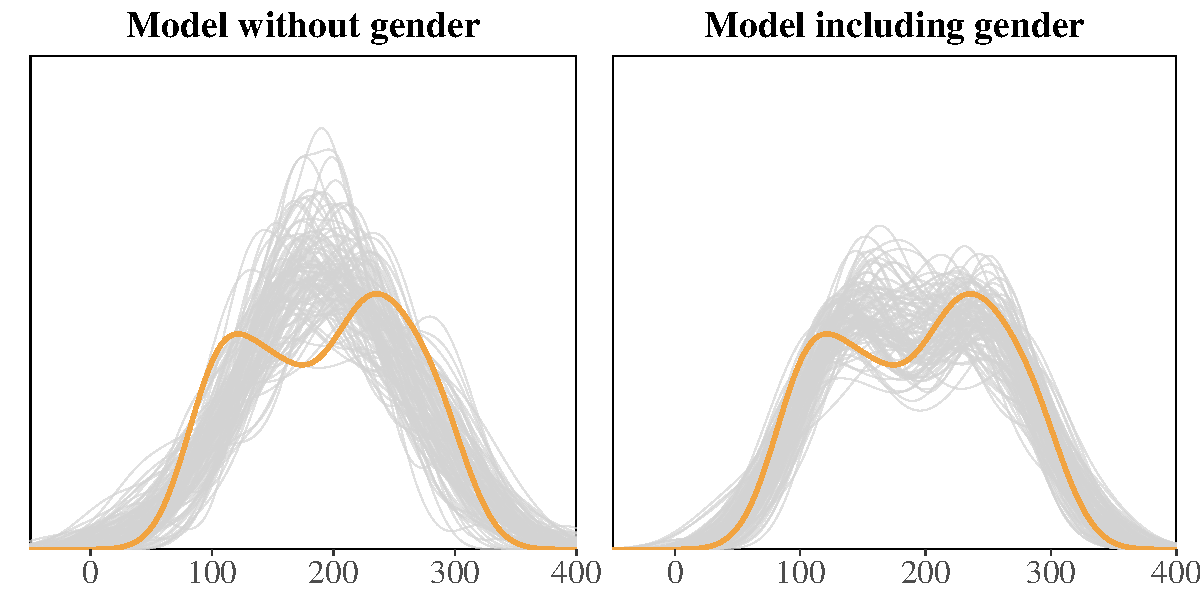
\includegraphics[width = 1\textwidth]{pics/pp_checks_plot.pdf}
    \caption{Output of the posterior predictive check for a model \textbf{without} the predictor \texttt{gender} in the left panel and a model \textbf{including} the predictor \texttt{gender} in the right panel. Red lines represent distribution of data, grey lines represent 100 posterior samples.}
    \label{fig:PPC}
\end{figure}

The model without gender overestimates the probability of very low and high pitch values, underestimates the probability of values that surround the two bumps and heavily overestimates the probability of values around 200 Hz.
The earlier model which takes \texttt{gender} into account looks quite a bit better (right panel). While still showing much uncertainty surrounding the two bumps in the observed distribution, it clearly captures the evidence better. 
\marginnote{The \texttt{pp\_check()} can take additional arguments that allow you to display posterior predictive distributions for individual parameters}

%\begin{figure}[]
%  \centering
%    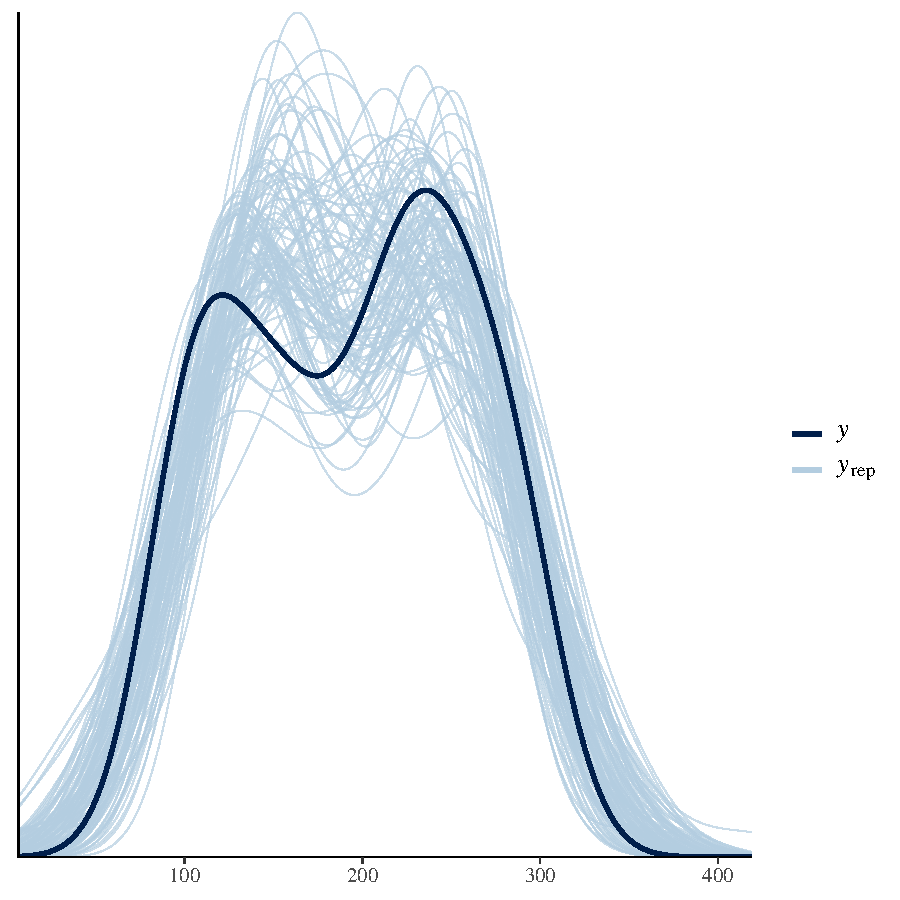
\includegraphics[width = 0.8\textwidth]{pics/pp_check_FE.pdf}
%    \caption{Output of the posterior predictive check for a model with the predictor \texttt{gender}. Orange line represents distribution of data, grey lines represent 100 posterior samples.}
%    \label{fig:PPC_with_gender}
%\end{figure}


\section{Adding random effects}

In our experiment, we measured pitch multiple times for each subject (since they produced
multiple sentences). We also have multiple measures for each sentence (as each sentence was
produced by multiple speakers). The observant reader might have already noticed this, but it is
probably worth reiterating that linear regression models make the crucial assumption that all
samples (data points) are independent of each other. But if two data points are produced by the
same participant, then observations will not necessarily be independent anymore. We need to
inform the model about these dependencies between observations. The way we’re going to handle
this is to add random effects to the model, just as we do in the frequentist framework. Random
effects are additional parameters that the Bayesian model estimates and that account for
dependencies between data points. The choice of the random effect structure is controversial.
This tutorial follows the approach advocated by \citet{barr2013random} to include the maximal
random effect structure justified by the design \citep[for a complementary view on random
effect specifications, see][]{matuschek2017balancing}. For our case here, we estimate how
individual sentences (\texttt{(1 | sentence)}) and individual subjects (\texttt{(1 | subject)})
differ in their overall pitch values (random intercepts). We also estimate how much pitch
values across sentences vary according to the context they appear in and according to the
gender of the speaker (as well as their interaction, i.e. \texttt{(0 + gender * context |
  sentence)}). This so-called by-sentence random slope allows the interaction term to vary
between sentences. In other words, the impact of the predictors gender and context (and their
interaction) might be different for different sentences. Finally, we estimate how much pitch
values vary across subjects as a function of context (\texttt{(0 +  context |
  subject)}). In other words, our model takes into
account that the context dependent effect on pitch might differ between individual speakers.

Running hierarchical random effect models with \textrm{brms} is very similar to the look and feel of non-Bayesian approaches. Here is the function call to the model.
The outcome of this model fit is shown below:

\begin{minipage}[]{1\textwidth}
\begin{lstlisting}[language=R]

# model including random intercepts and random slopes 
model_MaxRE = brm(formula = pitch ~ gender * context +
	(1 | sentence) + (1 | subject) + 
	(0 + gender * context | sentence) +
	(0 + context | subject),
	data = politedata, control = list(adapt_delta = 0.99)	)
\end{lstlisting}
\end{minipage}

\vspace{-0.5cm}

\begin{minipage}[]{1.5\textwidth}
\begin{rc}
 Family: gaussian 
  Links: mu = identity; sigma = identity 
Formula: pitch ~ gender * context + (1 + gender * context | sentence) + (1 + context | subject) 
   Data: politedata (Number of observations: 83) 
Samples: 4 chains, each with iter = 2000; warmup = 1000; thin = 1;
         total post-warmup samples = 4000

Group-Level Effects: 
~sentence (Number of levels: 7) 
                                   Estimate Est.Error l-95% CI u-95% CI Eff.Sample Rhat
sd(Intercept)                         21.60     10.11     6.94    47.11       1827 1.00
sd(genderM)                           10.65      8.59     0.41    30.40       2060 1.00
sd(contextpol)                        14.97     11.58     0.72    42.70       1526 1.00
sd(genderM:contextpol)                17.20     13.20     0.80    49.12       1785 1.00
cor(Intercept,genderM)                -0.22      0.44    -0.89     0.68       5035 1.00
cor(Intercept,contextpol)              0.02      0.42    -0.75     0.78       4760 1.00
cor(genderM,contextpol)               -0.06      0.45    -0.86     0.78       3019 1.00
cor(Intercept,genderM:contextpol)     -0.10      0.42    -0.81     0.73       4905 1.00
cor(genderM,genderM:contextpol)       -0.04      0.44    -0.83     0.78       3158 1.00
cor(contextpol,genderM:contextpol)    -0.15      0.44    -0.88     0.74       2897 1.00

~subject (Number of levels: 6) 
                          Estimate Est.Error l-95% CI u-95% CI Eff.Sample Rhat
sd(Intercept)                35.63     17.94    14.55    80.85       1643 1.00
sd(contextpol)                9.38      8.99     0.33    33.61       2508 1.00
cor(Intercept,contextpol)     0.05      0.58    -0.94     0.97       4544 1.00

Population-Level Effects: 
                   Estimate Est.Error l-95% CI u-95% CI Eff.Sample Rhat
Intercept            260.76     24.85   210.02   311.66       1557 1.00
genderM             -115.40     33.23  -181.79   -43.70       1438 1.00
contextpol           -27.53     12.96   -53.34    -2.40       2470 1.00
genderM:contextpol    16.21     16.90   -17.83    50.05       2441 1.00

Family Specific Parameters: 
      Estimate Est.Error l-95% CI u-95% CI Eff.Sample Rhat
sigma    25.01      2.37    20.88    30.09       3342 1.00

Samples were drawn using sampling(NUTS). For each parameter, Eff.Sample 
is a crude measure of effective sample size, and Rhat is the potential 
scale reduction factor on split chains (at convergence, Rhat = 1).
\end{rc}
\end{minipage}

\vspace{-0.5cm}

Lines 28--33 give the estimates of the fixed-effects coefficients. The mean estimates look very similar to the ones that we obtained in the fixed-effect only model. However, not surprisingly, our uncertainty surrounding these estimates is larger.  
We now also get information about the parameters implied by the specified random effect
structure. Lines 8--20 cover the by-sentence random effects, lines 22--26 cover the by-subject
random effects.

To check the probability of our hypotheses of interest, we can use the \texttt{faintr} package again, in conjunction with the convenience function for the specific hypotheses relevant for this tutorial:

\begin{minipage}[]{\textwidth}
\begin{rc}
> get_posterior_beliefs_about_hypotheses(model_MaxRE)
# A tibble: 3 x 2
  hypothesis                      probability
  <chr>                                 <dbl>
1 Female-polite < Female-informal       0.982
2 Male-polite < Male-informal           0.808
3 Male-informal < Female-polite         0.985
\end{rc}
\end{minipage}

\vspace{-0.5cm}

When we compare these values to the simpler model above, we can see that the evidence for our
hypotheses seems a bit weaker for the maximal random effect model. This is not surprising
because the simpler model assumed independence where there was none and therefore
underestimated the variance. Speech is a messy aspect of human behavior. Speakers differ quite
drastically in their pronunciation and even the same speaker varies a lot in how they speak.
If we do not inform our model about these sources of variation, we might end up being overly confident in our results.


\section{Reporting the results}
How do we report our analysis and our results in a Bayesian framework? There is no gold
standard. But the following is one example for how to do it.

\paragraph{Description of analysis.}

``We fitted Bayesian hierarchical linear models to pitch values as a function of dummy-coded
factors \textsc{gender} (reference level ``female''), and \textsc{context} (reference level
``informal'') and their two-way interaction, using the Stan modeling language
\citep{carpenter2016stan} and the package \emph{brms} \citep{buerkner2016brms}. The models
included maximal random-effect structures justified by the design, allowing the predictors of
interest and their interactions to vary by participants (\textsc{context}) and sentences
(\textsc{gender}, \textsc{context}). We used the default priors of the \texttt{brms} package,
namely a Student's $t$-distribution ($\nu = 3$, $\mu = 204$, $\sigma = 83$) for the mean of the
reference cell (female speakers in an informal context), a Student's $t$-distribution ($\nu =
3$, $\mu = 0$, $\sigma = 83$) for standard deviation for the likelihood function, and unbiased
priors for regression coefficients. We used the \textit{brms} package's default priors for
standard deviations of random effects (a Student's $t$-distribution with $\nu = 3$, $\mu = 0$
and $\sigma = 20$), as well as for correlation coefficients in interaction models (LKJ $\eta =
1$).

Four sampling chains ran for 2000 iterations with a warm-up period of 1000 iterations for each
model, thereby yielding 4000 samples for each parameter tuple. For all relevant cell means and differences
between them, we report the expected values under the posterior distribution and their 95\%
credible intervals (CIs). For differences between cells, we also report the posterior
probability that a difference $\delta$ is bigger than zero. If a hypothesis states that
$\delta >0$, we judge there to be \emph{compelling evidence} for this hypothesis if zero is (by
a reasonably clear margin) not included in the 95\%\,CI of $\delta$ and the posterior $P(\delta
>0)$ is close to one.

\paragraph{Description of results.}  

Female speakers produced higher voice pitch in informal contexts ($\mathbb{E}(\mu_{\text{fem,
    inf}}) = 261$, CI = [210, 312]) than in polite contexts ($\mathbb{E}(\mu_{\text{fem,
    pol}}) = 233$, CI = [179, 288]). There is compelling evidence for this difference
($\mathbb{E}(\mu_{\text{fem, inf}} - \mu_{\text{fem, pol}}) = 28$, CI = [2, 53], $P(§\delta
> 0) = 0.982$). We conclude that the data and the model support H1.
%
\marginnote{Notation $\mathbb{E}(\cdot)$ is shorthand for the expectation (mean) of the
  posterior distribution of some (possibly derived) quantity of interest.}

Male speakers also produced higher voice pitch in informal contexts
($\mathbb{E}(\mu_{\text{male, inf}}) = 145$, CI = [94, 191]) than in polite contexts
($\mathbb{E}(\mu_{\text{male, pol}}) = 134$, CI = [77, 184]). However, there is no sufficient
evidence that this difference is larger than zero ($\mathbb{E}(\mu_{\text{male, inf}} - \mu_{\text{male, pol}}) =$ 11, CI =
[-16, 40], $P(\delta > 0) = 0.809$). We conclude that the data and the model do not
support H2.

Female speakers in polite contexts produced higher voice pitch ($\mathbb{E}(\mu_{\text{fem,
    pol}}) = 233$, CI = $[179, 288]$) than male speakers in informal contexts
($\mathbb{E}(\mu_{\text{male, inf}}) = 145$, CI = $[94, 191]$). There is compelling
evidence that the difference between these cells is larger than zero ($\mathbb{E}(\mu_{\text{fem,
    pol}} - \mu_{\text{male, inf}}) = $ 86, CI = [18, 162], $P(\delta >
0) = 0.985$). We conclude that the data and the model support H3."


\section{Other forms of Bayesian inference}

Alright, you made it! We have learned the basic reasoning behind Bayesian parameter estimation,
we learned about priors and how to specify them, we learned how to criticize our models and how
to write up our results. Phewww, if you feel a little overwhelmed by now, don't worry, it will
come to you. Before we send you off into the Bayesian data analysis world, we would like to mention a couple of things that we were not able to cover here.

There are three major things we can do with models and data in Bayesian data analysis, two of which we have already seen:

\begin{enumerate}
\item \textbf{parameter inference}: we consider one model, (tentatively) assume that this model is true, and ask what we should believe about its parameters (given the data);
\item \textbf{model criticism}: we consider one model and ask whether this model is sufficient to deal with the data at hand; we can do that before showing the model any of the data, or after feeding it with some or all of the data;
\item \textbf{model comparison} we consider at least two models and we ask which of these models (plural!) is better at explaining the data.
\end{enumerate}

So far, we have dealt with parameter inference and model criticism. In fact, we used parameter inference to test our research hypotheses, and we used model criticism as a sanity check to
make sure that the one model we used was adequate.

This tutorial focused on parameter estimation because it's simple and very familiar to those
who have used null hypothesis significance testing in a frequentist framework before. But if
you dive deeper into Bayesian data analysis, you will quickly discover that there are good
arguments \citep[e.g.][]{VandekerckhoveMatzke2015:Model-Compariso} for an approach to
hypothesis testing that is based on Bayesian model comparison in terms of so-called
\textbf{Bayes factors} \citep{Jeffreys1961:Theory-of-Proba,KassRaftery1995:Bayes-Factors} or
cross-validation like \textbf{Leave-One-Out (LOO)} \citep{VehtariGelman2016:Practical-Bayes}.
These techniques lead us too deep into the rabbit hole of Bayesian inference for today, but we
can offer some (hopefully) helpful departure points for further reading.

\section{Further reading}

The textbook by \citet{GelmanCarlin2014:Bayesian-Data-A} is a standard reference for Bayesian
data analysis. \citet{Kruschke2011:Doing-Bayesian-} provides a less technical introduction to
Bayesian methods. \citet{McElreath2016:Statistical-Ret} is both an excellent introduction to
core concepts of statistical analysis and and excellent point of departure into Bayesian
analyses.
%
\marginnote{A. Solomon Kurz has an online book based on
  \citet{McElreath2016:Statistical-Ret}, which uses the same tools as we did here, namely the
  \emph{tidyverse} and the \emph{brms} packages: \url{https://bookdown.org/ajkurz/Statistical_Rethinking_recoded/}}.
There are many other useful tutorials to Bayesian analysis using \emph{brms}, some of which are
technically a little bit more involved \citep[e.g.][]{SorensenHohensteinb2016:Bayesian-linear}.
If you want to explore Bayesian approaches to data analysis with a graphical user interface, check out JASP: \url{https://jasp-stats.org}. 








\printbibliography[heading=bibintoc]

\end{document}
